
\documentclass[11pt]{article}
\usepackage{amsmath, amssymb, amsthm}
\usepackage{geometry}
\usepackage{graphicx}
\geometry{margin=1in}
\title{Foundations of Machine Learning -- Lecture 6 Notes}
\author{}
\date{}
\setlength{\parindent}{0pt}

\begin{document}
\maketitle

\section*{Dimensionality Reduction}
We care about this to overcome the curse of dimensionality, and to better compress our data.
It also leads to simpler data visualization and denoising.

\begin{figure}[h!]
	\centering
	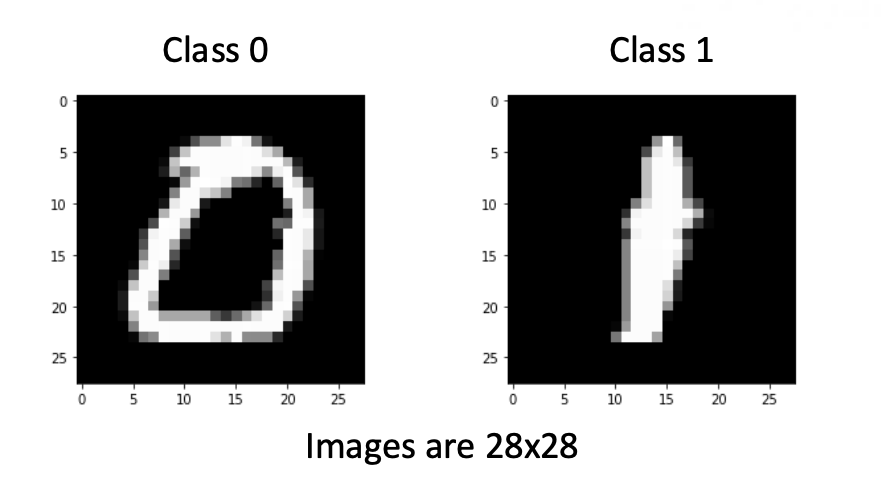
\includegraphics[width=0.6\textwidth]{../imgs/MNIST.png}
	\caption{MNIST handwritten classification dataset}
\end{figure}

We can vectorize the dataset:
\[
	x^{(i)} \in \mathbb{R}^{784}
	\quad
	y^{(i)} \in {0,1}
\]

One option to reduce dims is to use principle components, and only track 2 features of the images, one being how line-like it is and another for how curved it is.

\begin{figure}[h!]
	\centering
	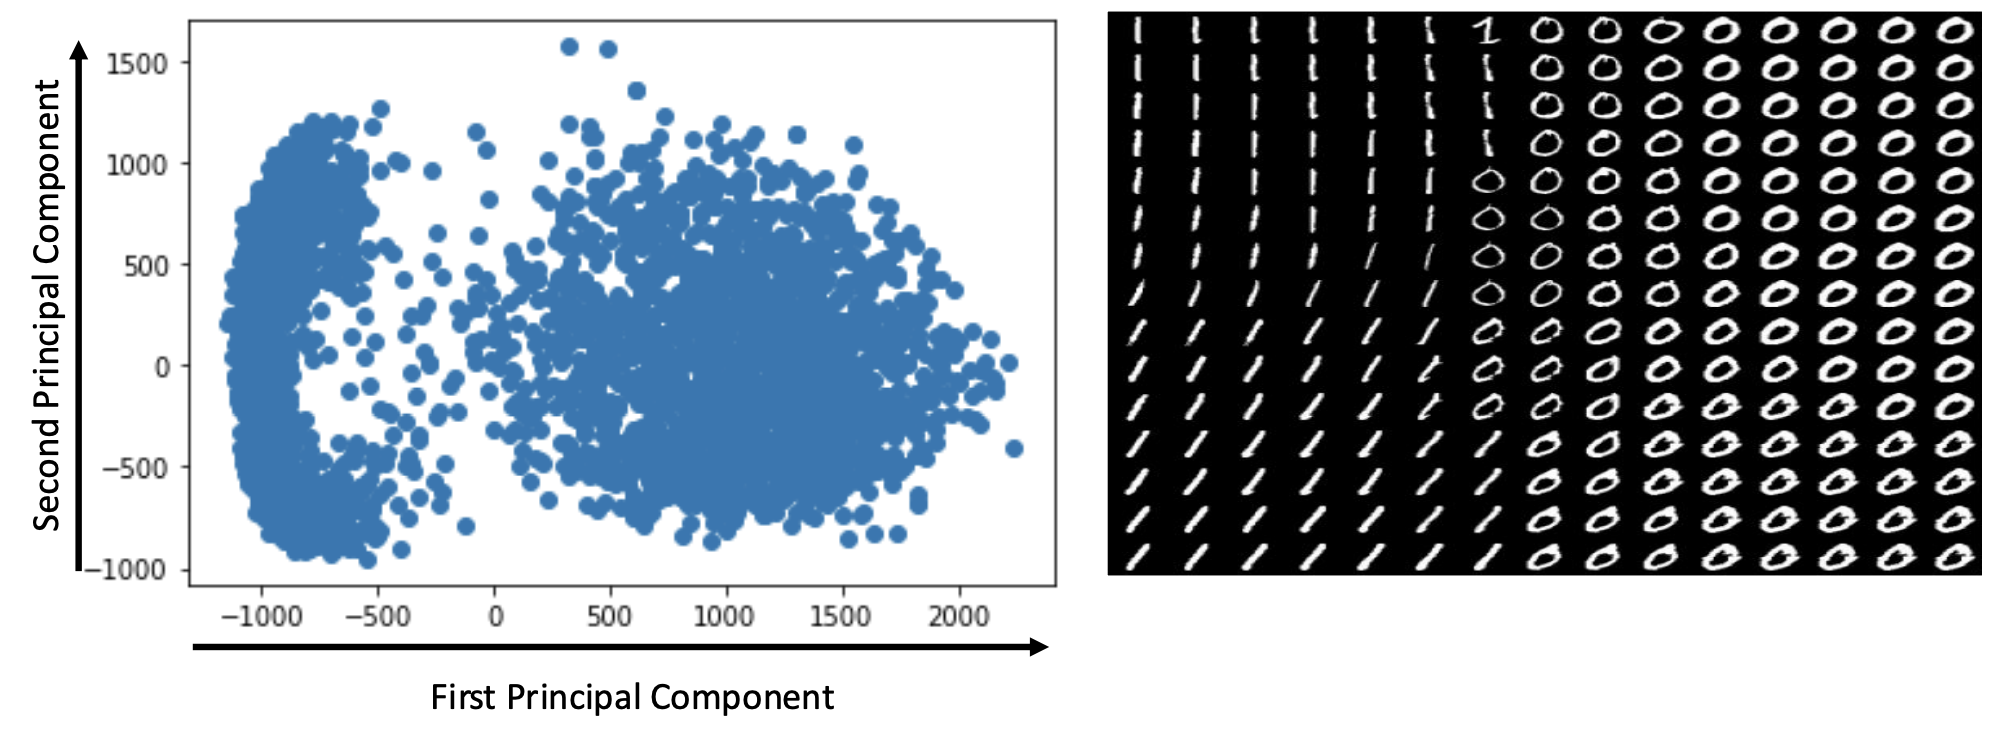
\includegraphics[width=0.6\textwidth]{../imgs/pcomps.png}
	\caption{MNIST handwritten classification dataset}
\end{figure}

\pagebreak

Whatever method we choose the main goal is for our reduced data to preserve as much information as possible.
\[
	f: \mathbb{R}^d \rightarrow \mathbb{R}^k \quad k<d
\]
\[
	x \in \mathbb{R}^d
\]
\[
	z = f(x) \in \mathbb{R}^k
\]

We may want to be able to recover x from z as closely as possible.

\subsection*{Maximizing Variance}

Find $w$ such that it maximizes the variance of the projected data

We have data
\[
	x = \{x_1, x_2,\dots, x_N\in \mathbb{R}^d\}
\]

Our reduced data is
\[
	\left\{ z_i =w^Tx_i \right\}_{i=1}^{N}
\]


Let’s first calculate the mean of the reduced data:
\[
	\bar{z} = \frac{1}{N} \sum_{i=1}^{N} z_i
	= \frac{1}{N} \sum_{i=1}^{N} \mathbf{w}^T \mathbf{x}_i
	= \mathbf{w}^T \left( \frac{1}{N} \sum_{i=1}^{N} \mathbf{x}_i \right)
	= \mathbf{w}^T \bar{\mathbf{x}}
\]
Then the variance of the reduced data is:
\[
	\mathrm{var} = \frac{1}{N} \sum_{i=1}^{N} (z_i - \bar{z})^2
	= \frac{1}{N} \sum_{i=1}^{N} \left( \mathbf{w}^T (\mathbf{x}_i - \bar{\mathbf{x}}) \right)^2
\]

\[
	\text{var} = \frac{1}{N} \sum_{i=1}^{N} \left(w^T(x_i - \bar{x})\right)^2
	= \frac{1}{N} \sum_{i=1}^{N} w^T(x_i - \bar{x})(x_i - \bar{x})^T w
\]

\[
	= w^T \left( \frac{1}{N} \sum_{i=1}^{N} (x_i - \bar{x})(x_i - \bar{x})^T \right) w
	= w^T S w
\]

\[
	\text{Therefore maximizing the variance can be written as:}
\]

\[
	\max_{w} \quad w^T S w \quad \text{s.t.} \quad w^T w = 1
\]
High variance: Data points are well spread and captures meaningful differences between samples
Low variance: Almost constant and carries little distinction across data

\medskip

We set the constraint to be $w^tw = 1$ so that our w corresponds to an actual direction change instead of just bumping magnitude.

Any solution to this must satisfy:

\[
	S w = \lambda w, \qquad w^T w = 1
\]

\medskip

But we want to find the eigenvector that maximizes $w^T S w$

\pagebreak

Some characteristics of eigenvectors:
\begin{itemize}
	\item $\|v_i\| = 1$
	\item $v_i^T v_j = 0,\;\; \forall i \ne j$ \quad (orthogonal)
\end{itemize}

\medskip
Covariance matrix $S$ is real and symmetric (PSD), so it can be uniquely decomposed as:

\[
	S = \sum_i \lambda_i v_i v_i^T
\]

Multiply both sides by eigenvector $v_k$:

\[
	v_k^T S v_k = \lambda_k
\]

\bigskip

Therefore, $w$ should be the first eigenvector (largest eigenvalue) of $S$.


\subsection*{Minimizing Reconstruction Error}

In order to reconstruct from $z \rightarrow x$ we see the following:

\[
	\hat{x} = w w^T x
\]

Now we can write the reconstruction error as:

\begin{align}
	\frac{1}{N} \sum_{i=1}^{N} \left\| \hat{x}^{(i)} - x^{(i)} \right\|^2
	 & = \frac{1}{N} \sum_{i=1}^{N} \left\| ww^T x^{(i)} - x^{(i)} \right\|^2
\end{align}

This is equivalent to maximizing the variance! see:
\[
\begin{aligned}
\arg\min_{w} \;& \frac{1}{N} \sum_{i=1}^{N} \left\| ww^T x^{(i)} - x^{(i)} \right\|^2 \\
= \arg\min_{w} \;& \frac{1}{N} \sum_{i=1}^{N} (ww^T x_i - x_i)^T (ww^T x_i - x_i) \\
= \arg\min_{w} \;& \frac{1}{N} \sum_{i=1}^{N} x_i^T ww^T ww^T x_i - 2x_i^T ww^T x_i \\
= \arg\min_{w} \;& -\frac{1}{N} \sum_{i=1}^{N} x_i^T ww^T x_i \\
= \arg\min_{w} \;& - w^T \left( \frac{1}{N} \sum_{i=1}^{N} x_i x_i^T \right) w \\
= \arg\max_{w} \;& w^T S w
\end{aligned}
\]


\subsection*{Transpose Trick}

Standard covariance matrix:
\[
S = \frac{1}{N}XX^T \in \mathbb{R}^{DXD}
\]

We then calculate the eigen decomposition of a dxd matrix

If d $>>$ n we can instead use this:
\[
G = \frac{1}{N}X^TX \in R^{NXN}
\]

This allows us to calculate the eigenvectors in a smaller space and then scale to our original space.

\subsection*{Linear Discriminant Analysis (LDA)}
Remember that PCA is a unsupervised technique, this means that it does not care weather a data point is of a particular class.

\medskip

Distance between class means 
\[
\begin{aligned}
&= \frac{1}{K} \sum_{k} \left( w^T \mu^{(k)} - w^T \bar{\mu} \right)^2 \\
&= \frac{1}{K} \sum_{k} \left( w^T (\mu^{(k)} - \bar{\mu}) \right)^2 \\
&= w^T \left( \frac{1}{K} \sum_{k} (\mu^{(k)} - \bar{\mu})(\mu^{(k)} - \bar{\mu})^T \right) w \\
&= w^T S_b w
\end{aligned}
\]

Within class variance
\[
\begin{aligned}
&= \frac{1}{N} \sum_{k} \sum_{i \in \mathcal{C}_k} \left( w^T x^{(i)} - w^T \mu^{(k)} \right)^2 \\
&= \frac{1}{N} \sum_{k} \sum_{i \in \mathcal{C}_k} \left( w^T (x^{(i)} - \mu^{(k)}) \right)^2 \\
&= w^T \left( \frac{1}{N} \sum_{k} \sum_{i \in \mathcal{C}_k} (x^{(i)} - \mu^{(k)})(x^{(i)} - \mu^{(k)})^T \right) w \\
&= w^T S_w w
\end{aligned}
\]

We want to maximize the distance between class means and minimize the within class variance.


\begin{figure}[h!]
	\centering
	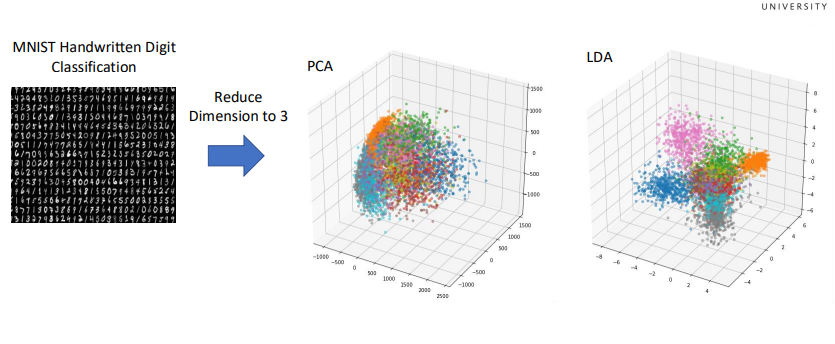
\includegraphics[width=0.6\textwidth]{../imgs/pcavlda.png}
	\caption{MNIST handwritten classification dataset}
\end{figure}

\subsection*{Auto-Encoder (AE)}

This is a nonlinear mapping to compress input $x \in \mathbb{R}^d$ into 
a lower-dimensional latent code $z \in \mathbb{R}^k$, and then reconstruct $x$ from $z$.

\[
\text{Encoder:} \quad z = \phi(x), \qquad \phi: \mathbb{R}^d \rightarrow \mathbb{R}^k
\]
\[
\text{Decoder:} \quad \hat{x} = \psi(z), \qquad \psi: \mathbb{R}^k \rightarrow \mathbb{R}^d
\]

The objective is to minimize reconstruction error:
\[
\min_{\phi,\psi} \; \mathbb{E}_{x} \left[ \|x - \hat{x}\|^2 \right] 
= \mathbb{E}_{x} \left[ \|x - \psi(\phi(x))\|^2 \right]
\]


\begin{itemize}
    \item Unlike PCA, the mappings $\phi$ and $\psi$ can be \textit{nonlinear}.
    \item Allows learning of \textbf{curved or nonlinear manifolds} in data.
    \item PCA is a \textbf{special case} of AE when $\phi$ and $\psi$ are linear.
\end{itemize}



\subsection{Canonical Correlation Analysis (CCA)}
This is a cross decomposition algorithm for example:

\medskip

\begin{itemize}
    \item Measurement 1: $x^{(i)} = \text{[Gender, Age, Height, Weight, Education, etc.]}$ \\ Measurement 2: $y^{(i)} = \text{[Net Worth, Credit Score, Annual Income, etc.]}$
    \item Measurement 1: Video \\ Measurement 2: Audio
    \item Measurement 1: English words \\ Measurement 2: German translations
\end{itemize}

Data set: \(\{(x^{(i)}, y^{(i)})\}_{i=1}^N\)

\medskip

This method jointly finds a dimentionality reduction for X and Y into the same embedding space such that the correlation between the embedded x and y is maximized.

\begin{figure}[h!]
	\centering
	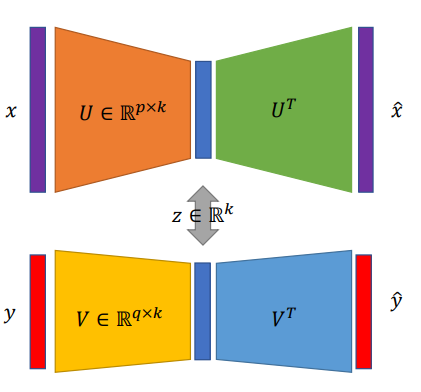
\includegraphics[width=0.6\textwidth]{../imgs/cca.png}
	\caption{MNIST handwritten classification dataset}
\end{figure}


\begin{figure}[h!]
	\centering
	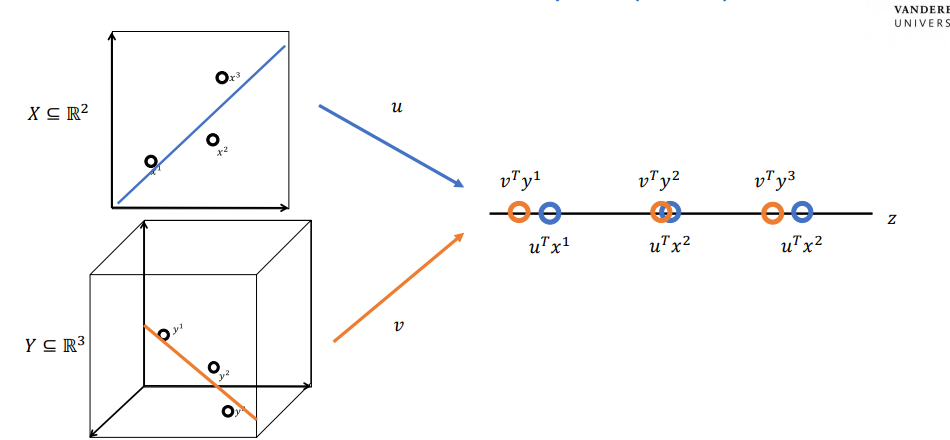
\includegraphics[width=0.6\textwidth]{../imgs/cca-proj.png}
	\caption{MNIST handwritten classification dataset}
\end{figure}

\paragraph{Formulation}

First, we define our objective as maximizing the (centered) cross-correlation:
\[
\max_{u,v} \; \frac{1}{N} \sum_{i=1}^N 
\left(u^\top (x^{(i)} - \bar{x})\right)
\left(v^\top (y^{(i)} - \bar{y})\right)
\]

Then rewrite the inner product more compactly:
\[
= \max_{u,v} \; \frac{1}{N} \sum_{i=1}^N 
u^\top (x^{(i)} - \bar{x}) (y^{(i)} - \bar{y})^\top v
\]

Then pull \(u\) and \(v\) outside the summation:
\[
= \max_{u,v} \; u^\top 
\left(
\frac{1}{N} \sum_{i=1}^N (x^{(i)} - \bar{x})(y^{(i)} - \bar{y})^\top
\right)
v
\]

Define the cross-covariance matrix:
\[
S_{xy} = \frac{1}{N} \sum_{i=1}^N (x^{(i)} - \bar{x})(y^{(i)} - \bar{y})^\top
\quad \Rightarrow \quad
\max_{u,v} \; u^\top S_{xy} v
\]

Finally, constrain the variances to avoid trivial solutions:
\[
\max_{u,v} \; u^\top S_{xy} v
\quad \text{s.t.} \quad
u^\top S_{xx} u = v^\top S_{yy} v = 1
\]

\begin{itemize}
    \item \textbf{Lagrangian:} \quad
    \[
    \mathcal{L} = -u^\top S_{xy} v 
    + \frac{\lambda_1}{2} (u^\top S_{xx} u - 1)
    + \frac{\lambda_2}{2} (u^\top S_{yy} u - 1)
    \]

    \item \textbf{Solution:} \quad
    \[
    \left(S_{yy}^{-1} S_{xy} S_{xx}^{-1} S_{xy}^\top \right) v = \lambda^2 v
    \quad \text{where} \quad \lambda := \lambda_u \lambda_v
    \]
\end{itemize}

Once CCA has learned a shared latent space $z \in \mathbb{R}^k$ using $u$ and $v$, we can move back and forth between domains.
This allows us to reconstruct y from x and vise versa!

\begin{figure}[h!]
	\centering
	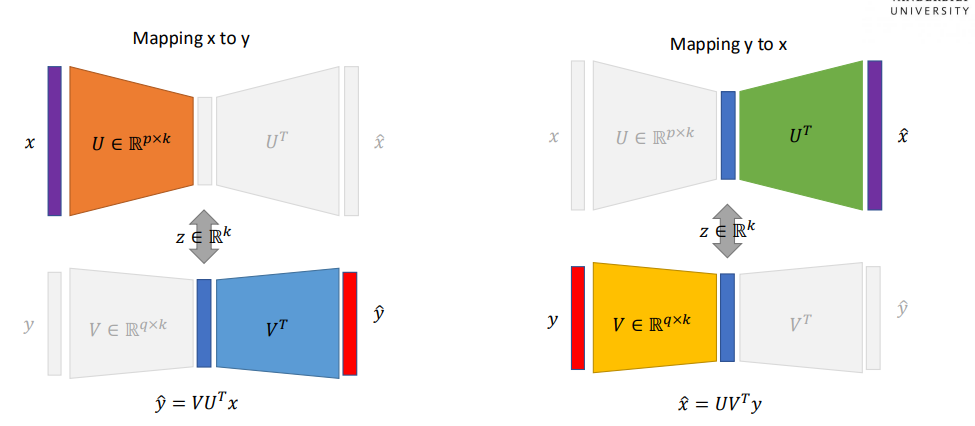
\includegraphics[width=0.6\textwidth]{../imgs/cca-translation.png}
	\caption{MNIST handwritten classification dataset}
\end{figure}



\end{document}

